\documentclass[10pt]{beamer}
\usepackage{appendixnumberbeamer}
\usetheme[progressbar=frametitle]{metropolis}
\usepackage[utf8]{inputenc}
\usepackage{graphicx}
\usepackage{booktabs}
\usepackage{multicol}
\usepackage{multirow}
\usepackage{xspace}
\usepackage{color}
\usepackage{underscore}
\usepackage{url}
\usepackage{verbatim}
\usepackage{listings}
\lstdefinestyle{ErrorStyle}{
   identifierstyle=\color{red},
   numberstyle=\tiny\color{yellow},
   literate={0}{{{\color{red}0}}}1
            {1}{{{\color{red}1}}}1
            {2}{{{\color{red}2}}}1
            {3}{{{\color{red}3}}}1
            {4}{{{\color{red}4}}}1
            {5}{{{\color{red}5}}}1
            {6}{{{\color{red}6}}}1
            {7}{{{\color{red}7}}}1
            {8}{{{\color{red}8}}}1
            {9}{{{\color{red}9}}}1
            {.0}{{{\color{red}.0}}}2
            {.1}{{{\color{red}.1}}}2
            {.2}{{{\color{red}.2}}}2
            {.3}{{{\color{red}.3}}}2
            {.4}{{{\color{red}.4}}}2
            {.5}{{{\color{red}.5}}}2
            {.6}{{{\color{red}.6}}}2
            {.7}{{{\color{red}.7}}}2
            {.8}{{{\color{red}.8}}}2
            {.9}{{{\color{red}.9}}}2
            {(}{{\color{red}{(}}}{1}
            {)}{{\color{red}{)}}}{1}
            {-}{{\color{red}{-}}}{1}
            {:}{{\color{red}{:}}}{1}
   }
\lstdefinestyle{CStyle}{
   backgroundcolor=\color{black},
   commentstyle=\color{green},
   keywordstyle=\color{blue},
   identifierstyle=\color{green},
   numberstyle=\tiny\color{yellow},
   stringstyle=\color{purple},
   basicstyle=\footnotesize,
   breakatwhitespace=false,
   breaklines=true,
   captionpos=b,
   keepspaces=true,
   numbers=left,
   numbersep=5pt,
   showspaces=false,
   showstringspaces=false,
   showtabs=false,
   tabsize=2,
   language=C,
   literate={0}{{{\color{magenta}0}}}1
            {1}{{{\color{magenta}1}}}1
            {2}{{{\color{magenta}2}}}1
            {3}{{{\color{magenta}3}}}1
            {4}{{{\color{magenta}4}}}1
            {5}{{{\color{magenta}5}}}1
            {6}{{{\color{magenta}6}}}1
            {7}{{{\color{magenta}7}}}1
            {8}{{{\color{magenta}8}}}1
            {9}{{{\color{magenta}9}}}1
            {.0}{{{\color{magenta}.0}}}2
            {.1}{{{\color{magenta}.1}}}2
            {.2}{{{\color{magenta}.2}}}2
            {.3}{{{\color{magenta}.3}}}2
            {.4}{{{\color{magenta}.4}}}2
            {.5}{{{\color{magenta}.5}}}2
            {.6}{{{\color{magenta}.6}}}2
            {.7}{{{\color{magenta}.7}}}2
            {.8}{{{\color{magenta}.8}}}2
            {.9}{{{\color{magenta}.9}}}2
            {(}{{\color{yellow}{(}}}{1}
            {)}{{\color{yellow}{)}}}{1}
   }
\usecolortheme{albatross}
\setbeamercolor{normal text}{bg=black, fg=white}
\setbeamerfont{normal text}{size=3pt}
\newcommand{\themename}{\textbf{\textsc{metropolis}}\xspace}
\title{\small Instituto Tecnológico de Costa Rica \newline 
        Compiladores e Intérpretes \newline 
        Proyecto2: Análisis Sintáctico \newline 
        Prof: Francisco Torres Rojas} 
\date{II Semestre 2017} 
\author{\large Jason Barrantes A. 2015048456 \newline 
                 Randy Morales G. 2015085446 \newline} 

\def\ContinueLineNumber{\lstset{firstnumber=last}} 
\def\StartLineAt#1{\lstset{firstnumber=#1}} 
\let\numberLineAt\StartLineAt 
\begin{document} 
\maketitle 
\begin{frame}[fragile]{CONTENIDOS} 
    \setbeamertemplate{section in toc}[sections numbered] 
    \tableofcontents 
\end{frame} 

\section{BISON Y FASE DE PARSING}
\begin{frame}[fragile]{BISON} 
    BISON es un proyecto creado por GNU, por lo que es la versión libre de YACC. 
    Es un programa que genera analizadores sintácticos con propósitos generales. 
    Este está disponible para cualquier sistema operativo y se usa acompañado de \textbf{Flex}. 
    Convierte la descripción de un lenguaje, escrita con una gramática libre de contexto (CFG), 
    en un programa en C, C++ o Java que realiza el análisis sintáctico. Para la utilización de Bison, 
    es necesaria tener la gramática a analizar. \newline 
    
    Al compilarse el archivo Bison se generan dos archivos , un \textbf{archivo .h} y otro .c. 
    El archivo .h debe incluirse en el archivo de Lex/Flex. 
\end{frame} 

\begin{frame}[fragile]{ELEMENTOS} 
    El archivo de codificación de Bison tiene cuatro secciones: 
    
    \%{ 
    
    Declaraciones C 
    
    \%} 
    
    Declaraciones Yacc/Bison 
    
    \%Declaracion de Token 
    
    \%\% 
    
    Reglas de la gramática 
    
    \%\% 
    
    Código C 
\end{frame} 
\begin{frame}[fragile]{ELEMENTOS} 
    \%\{, \%\} sirven para delimitar el encabezado, donde usualmente se colocan bibliotecas 
    
    \%\% sirven para indicar cuales son las reglas 
    
    Y por último la programación en C o llamadas a funciones en caso de ser necesario. 
    
    \%Token Se utiliza para definir los símbolos no terminales (tokens) de la gramática. 
    
    \%token NOMBRE_TOKEN 
    
    Por convenio, los nombres de los tokens se escriben en mayúsculas y se pueden agrupar varios  
    tokens en una línea si tienen en mismo tipo. 
\end{frame} 

\begin{frame}[fragile]{CREADORES} 
    \begin{columns}[T] 
        \begin{column}{.5\textwidth} 
            \begin{block}{ } 
                Bison fue escrito en un principio por Robert Corbett; Richard Stallman lo hizo 
                compatible con Yacc y Wilfred Hansen de la Carnegie Mellon University añadió soporte 
                para literales multicaracter y otras características. 
            \end{block} 
        \end{column} 
        \begin{column}{.5\textwidth} 
            \begin{block}{Richard Stallman} 
                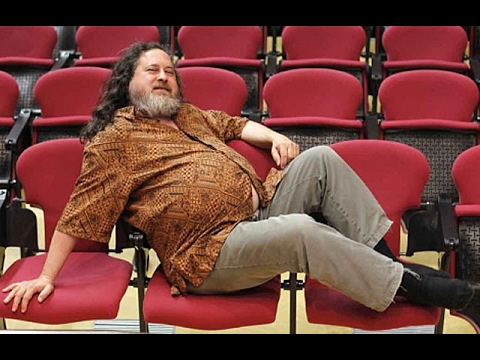
\includegraphics[width=6cm,height=4cm]{stallman} 
            \end{block} 
        \end{column} 
    \end{columns} 
\end{frame} 

\begin{frame}[fragile]{Parsing} 
    El parsing es la segunda fase de un compilador. La fase de parsing es el proceso donde se toma 
    el conjunto de tokens producidos por la fase de análisis léxico y se genera un 
    \textbf{árbol de sintaxis}. Luego este se revisa de acuerdo a la gramática formal del 
    lenguaje definido y se verifica que las expresiones construidas por el arreglo de tokens 
    sean sintacticamente correctos. \newline 
\end{frame} 

\section{CÓDIGO FUENTE} 
    \begin{lstlisting}[style=CStyle] 





                     static signed char a[] = {0x69,
                   110, 118, 97, 108, 105,  0x64, 1-1,
                 0x6d, 111, 118,  101, 1<<1<<1<<1<<1<<1,
                 114,  105, 0x6e,  103,  32, 'o'/3, 100,
                 32, 102, 114, 111,  0x6d, 32, 115, 116,
                 97, 100-001, 107, 32,37, 2*'2', '@'>>1,
                 116, ' + ' + ','w'-'W',115, 0x74,
                 97, 3*'!', 107, 'q' - 'Q', 37, 10*'\n',
                 10, 0}, * b = a + (1<<1<<1<<1), * w, x,
                 *q, c, r; int main(int d, char *e []) {
                 return q = (signed char *)(e+1+1), (r =
                 e[0] && e[1] ? 0 : 0 * puts (a) + 1) ||
                 (r = e[1<<1] && d != 1 <<1 && 0 * puts(
                 a) + 1) || e[1- -1] ||  (r = atoi(e[1])
                 < -0200 || atoi (e [1]) > 0x7f || ( x =
                 atoi( e[1] ) ) == 0 ? 0 * puts(a) + 1 :
                 0) || e [1- -1] || (x- -x > 1-1 ? (q[0]
                   = x, q[1] = q[3] = 1, q[2] = 2) : (
                     memset ( w = ( signed  char * )







                     malloc(-x), '1', -x), puts (w),
                   q[0] = x, q[1] = '0', q[2] = q[3] =
                 0)), r || (q[3] ? (c = 6 - q[1] - q[2],
                 (q[0] != 1) ? q[0]-- , d = q[2], q[2] =
                 c, main(2, e), c = q[2], q[2] = d, q[0]
                 ++ : 0, printf(b, q[0], q[1], q[2]), (q
                 [0] != 1) ? q[0]--, d = q[1],q[1] = c ,
                 main(2, e), c = q[1], q[1] = d, q[0] ++
                 : 0) : - 1 - q[0] - 1 == 0 ? (w[- x - 1
                 - (q[1] & 1 ^ 1)] = q[1], puts (w), w [
                 - x - 1 - (q[1] & 1)] = q[1], puts(w) )
                 : - 1 - q[0] == 0 ?  (w[- x - 1] = q[ 1
                   ], puts(w)) : (q[0] += 1 + ( q[1] & 1
                       ^ 1), main(2, e), q[0] -= 1 + ( q
                             [1] & 1 ^ 1), q[1] & 1 ? (q
                                [0]+=1+1,  q[1]^=1, main
                                (2, e), q[1]^=1, q[0]-=1
                                +1) : 0, w[q[0] - x] = q
                               [1], puts(w), q[1] & 1 ?
                             0 : (q[0]+=1+1, q[1]^=1,
                           main (2, e), q[1]^=1, q
                         [0]-=1+1), q[0] += 1 +
                      (q[1] & 1),main(2,e)
                  , q[0] -= 1 + (q[1]
                 & 1) ) ), r; }



                 float clauses(){
  float x = (0.5 + 
    1.23) - 2.145 * (7451 / 124.6) 
                      + 987 * 41 - 7123;
  float y = (0.5 + 1.23) - 2.145 * 
                (41 * 7 + (41256 * 4551)) + 9 * 11245 - 23;
  float z = (x * y) / (y * y) + 12000;
  float R = (0.5 + 1.23) - 2.145 * 
  
  
                  (7451 / 124.6) + 987 * 41 
                  - 7123;

  float P = (0.5 + 1.23) - 2.145 * (41 * 7 
            + (41256 * 4551)) + 9 * 11245 - 23;
  float G = (x * y) / (y * y) + 12000;
  float S3 = (0.5 + 1.23) - 2.145 * 
  
  
  (7451 / 124.6) + 987 * 41 - 7123;

  float A0 = (0.5 + 1.23) - 2.145 * (41 * 7 + 
                                      (41256 * 4551)) + 9 * 11245 - 23;
  float P1 = (x * y) / (y * y) + 12000;

  float R0 = (0.5 + 1.23) - 
  2.145 * (7451 / 124.6) + 987 * 41 - 7123;

  float I = (0.5 + 1.23) - 2.145 * (41 * 7 + (41256 * 4551)) 
  
  
                                              + 9 * 11245 - 23;
  float S = (x * y) / (y * y) + 12000;
  float S1 = (0.5 + 1.23) - 2.145 * 
  
  
  (7451 / 124.6) + 987 * 41 - 7123;
  float A = (0.5 + 1.23) - 2.145 * (41 * 
    
    
    7 + (41256 * 4551)) + 9 * 11245 - 23;
  float z1 = (x * y) / (y * y) + 12000;
  float x2 = (0.5 + 1.23) - 2.145 * 
  
  
  (7451 / 124.6) + 987 * 41 - 7123;
  float y3 = (0.5 + 1.23) - 2.145 * 
  
                      (41 * 7 + (41256 * 4551)) + 9 * 11245 - 23;
  
  
                      float z4 = (x * y) / (y * y) + 12000;

  return x + y + z + R + P + G + S3 + A0 + P1;
}


void include(){
char *step0 = "pixa"; char *makeF0 = "Adapted to the files";  



  char *splint0 = ""; 
char *step1 = "pixa"; 


            char *makeF1 = "Adapted to the files";  
            char *splint1 = "know"; 
char *step2 = "pixa"; char *makeF2 = "Adapted to the files";  


char *splint2 = "know"; 
char *step3 = "pixa"; 


char *makeF3 = "Adapted to the files";  


      char *splint3 = "know"; 
char *step4 = "pixa"; char *makeF4 = "Adapted to the files";  


char *splint4 = "know"; 
}

static int check_type(){

          char *step0 = "pixa";
          
    char *makeF0 = "Adapted to the files";  char *splint0 = "know"; 
char *step1 = "pixa"; 

          char *makeF1 = "Adapted to the files";  
          
          
          
                    char *splint1 = "know"; 
char *step2 = "pixa"; 

char *makeF2 = "Adapted to the files";  

      char *splint2 = "know"; 
char *step3 = "pixa"; char *makeF3 = "Adapted to the files";  char *splint3 = "know"; 
char *step4 = "pixa"; char *makeF4 = "Adapted to the files";  char *splint4 = "know"; 
}

void count(){
int count0 = 0; int count1 = 0; int count2 = 0; int count3 = 0; 


          int count4 = 0; int count5 = 0; int count6 = 0;
int count10 = 0; 

          int count11 = 0; int count22 = 0; 


int count320 = 0; int count415 = 0; int count51 = 0; int count61 = 0;
int count20 = 0; int count21 = 0; 


int count325 = 0; int count330 = 0; int count421 = 0; int count52 = 0; int count62 = 0;
int count30 = 0; int count311 = 0;


int count32 = 0; int count340 = 0; int count33 = 0; int count53 = 0; int count63 = 0;
int count40 = 0; int count411 = 0; 



int count525 = 0; int count350 = 0; int count44 = 0; int count54 = 0; int count64 = 0;
int count50 = 0; int count512 = 0; int count626 = 0; int count360 = 0; int count45 = 0; int count55 = 0; int count65 = 0;
char *step0 = "pixa"; 


      char *makeF0 = "Adapted to the files";  char *splint0 = ""; 
char *step1 = "pixa"; char *makeF1 = "Adapted to the files"; 


        char *splint1 = "know"; 
char *step2 = "pixa"; char *makeF2 = "Adapted to the files";  



      char *splint2 = "know"; 
char *step3 = "pixa"; char *makeF3 = "Adapted to the files";  char *splint3 = "know"; 
char *step4 = "pixa"; char *makeF4 = "Adapted to the files";  char *splint4 = "know"; 
}

void printLexicalErrors(){
char *step0 = "pixa"; char *makeF0 = "Adapted to the files";  


    
                            char *splint0 = ""; 
char *step1 = "pixa"; char *makeF1 = "Adapted to the files";  


          char *splint1 = "know"; 
char *step2 = "pixa"; char *makeF2 = "Adapted to the files";  char *splint2 = "know"; 
char *step3 = "pixa"; char *makeF3 = "Adapted to the files";  

          char *splint3 = "know"; 
char *step4 = "pixa"; char *makeF4 = "Adapted to the files";  char *splint4 = "know"; 

}

int yywrap(){
int count0 = 0; int count1 = 0; 



              int count2 = 0; int count3 = 0; int count4 = 0; 
              
              
              
              
              
              
              
              int count5 = 0; int count6 = 0;
int count10 = 0; 



int count11 = 0; int 


        count22 = 0; int count320 = 0; 
        
        
        
        
          int count415 = 0; int count51 = 0; int count61 = 0;
int count20 = 0; int count21 = 0; 


int count325 = 0; int count330 = 0; int count421 = 0; int count52 = 0; int count62 = 0;
int count30 = 0; int count311 = 0; 


int count32 = 0; int count340 = 0; int count33 = 0; int count53 = 0; int count63 = 0;
int count40 = 0; int count411 = 0; int count525 = 0; 


          int count350 = 0; int count44 = 0; int count54 = 0;
                       int count64 = 0;
int count50 = 0; int count512 = 0; 


  int count626 = 0; int count360 = 0; int count45 = 0; int count55 = 0; int count65 = 0;
}

void printErrors(){
char *step2 = "pizza";
}

void write_infile

(char string)

        {
  int size = 
  
  
  
          100;
	char messageStore[100];
  for(int i=0; 
    
    
    i < size; i++){
    
                  messageStore[i] 
    
    
    
    = string;
	}
}

void luthor(){
  int r=0,x,y=0,n         =             0     ;
   char       v   [
   100    ]                   ,  s;
int t[100     ]                    ,
 u[100               ]     ;  u
     [                   0
]=ftell(stdin        )       ;
while((v    )                 )
    {t  [         r ]=
strlen                 (
  v);y=
    t[         r             ]
    >y             ?        t [
     r         ]    :   y;
 u[++r   ]     =      
ftell(stdin )   ;                          }
 while          (                    n
     <>              y        )
{for(x=0             ;         x
<r;x++) {                           s
  =' '       ;              
 if(n<             t        [
     x            ]     )    {
fseek(stdin    ,u       [     x    ]
    +n   ,  0 )                     ;
scanf("%c",                          &
                          s        )
      ;                             }
printf("%c",   s                       )
                               ;      }
printf("\n");                 n
    ++   ;            }
}

void initValues(){
  int ax0,bx0,cx0,dx0,ex0,fx0,gx0,
  hx0,ix0,jx0,kx0,lx0,mx0,nx0,ox0,
  px0,qx0,rx0,sx0,tx0,ux0,vx0,wx0,
  xx0,yx0,zx0;
  int ax1,bx1,cx1,dx1,ex1,fx1,gx1,
  hx1,ix1,jx1,kx1,lx1,mx1,nx1,ox1,px1,
              qx1,rx1,sx1,tx1,ux1,vx1,wx1,xx1,yx1,zx1;
  int ax2,bx2,cx2,dx2,ex2,fx2,gx2,
  hx2,ix2,jx2,                  kx2,lx2,mx2,nx2,ox2,px2,
  qx2,rx2,sx2,tx2,ux2,vx2,wx2,xx2,yx2,zx2;
  int ax3,bx3,cx3,dx3,ex3,fx3,gx3,
  hx3,ix3,jx3,kx3,lx3,mx3,nx3,ox3,px3,qx3,
  rx3,sx3,tx3,ux3,vx3,            wx3,xx3,yx3,zx3;
  int ax4,bx4,cx4,dx4,ex4,fx4,gx4,hx4,ix4,jx4,kx4,lx4,mx4,
    nx4,ox4,px4,qx4,rx4,sx4,tx4,ux4,vx4,wx4,xx4,yx4,zx4;
  int ax5,bx5,                  cx5,dx5,ex5,fx5,gx5,hx5,ix5,jx5,kx5,lx5,mx5,
  nx5,ox5,px5,qx5,rx5,sx5,tx5,ux5,vx5,wx5,xx5,yx5,zx5;
  int ax6,bx6,cx6,dx6,            ex6,fx6,gx6,hx6,ix6,jx6,kx6,lx6,mx6,
  nx6,ox6,px6,qx6,rx6,sx6,tx6,ux6,vx6,wx6,xx6,yx6,zx6;
  int ax7,bx7,cx7,dx7,ex7,        fx7,gx7,hx7,ix7,jx7,kx7,lx7,mx7,
  nx7,ox7,px7,            qx7,rx7,sx7,tx7,ux7,vx7,wx7,xx7,yx7,zx7;
  int ax8,bx8,cx8,dx8,ex8,fx8,gx8,hx8,ix8,jx8,kx8,lx8,mx8,
  nx8,ox8,px8,qx8,rx8,sx8,        tx8,ux8,vx8,wx8,xx8,yx8,zx8;
  int ax9,bx9,cx9,dx9,ex9,        fx9,gx9,hx9,ix9,jx9,kx9,lx9,mx9,
  nx9,ox9,px9,qx9,rx9,sx9,tx9,ux9,vx9,wx9,xx9,yx9,zx9;

char a19,b19,c19,
  d19,e19,,f19,g19,h19,i19,j19,
  
  
  
  k19,l19,m19,n19,o19,p19
  ,q19,r19,s19,t19,u19,v19,w19,x19,y19,z19;

 char af0,bf0,cf0,df0,,ef0,ff0,gf0,hf0,if0,
  
  
  jf01,kf0,lf0,mf0,nf0,of0;
  
  char a1,b1,c1,d1,e1,f1,g1,h1,i1,
  
  
  j11,k1,l1,m1,n1,o1,
  
  
  
    p1,q1,r1,s1,t1,u1,v1,w1,x1,y11,z1;
  char a2,b2,c2,d2,e2,f2,
  
  
  
  
            g2,h2,i2,j2,k2,l2,m2,n2,o2,p2,q2,r2,s2,t2,u2,v2,w2,x2,y2,z2;
  char a3,b3,c3,d3,e3,f3,g3,h3,i3,j3,
  k3,l3,m3,n3,o3,p3,q3,r3,s3,t3,u3,v3,w3,x3,y3,z3;
  char a4,b4,c4,d4,e4,f4,g4,h4,i4,j4,k4,
  
  
  l4,m4,n4,o4,p4,q4,
  
  
  
  
                  r4,s4,t4,u4,v4,w4,x4,y4,z4;
  char a5,b5,c5,d5,e5,                      f5,g5,h5,i5,j5,k5,l5,
  
  m5,n5,o5,p5,q5,
  
  
  
  r5,s5,t5,u5,v5,w5,x5,y5,z5;
  char a6,b6,c6,d6,e6,                  f6,g6,h6,i6,j6,k6,l6,m6,
  n6,o6,p6,q6,r6,
  
  s6,t6,u6,v6,w6,x6,y6,z6;
  char a7,b7,c7,d7,e7,
          f7,g7,h7,i7,j7,k7,
          l7,m7,n7,o7,p7,q7,r7,s7,t7,u7,v7,w7,x7,y7,z7;
  char a8,b8,c8,d8,e8,f8,g8,h8,i8,
  j8,k8,l8,m8,n8,o8,p8,q8,r8,s8,t8,u8,v8,w8,x8,y8,z8;
  char a9,b9,c9,
  d9,e9,f9,g9,h9,i9,j9,
  
  
  
  k9,l9,m9,n9,o9,p9
  ,q9,r9,s9,t9,u9,v9,w9,x9,y9,z9;




  char a0,b0,c0,d0,e0,
  
  
  f0,g0,h0,i0,j00,k0,l0,m0,n0,o0,
                                p0,q0,r0,s0,t0,u0,v0,w0,x0,y00,z0;
  
  a0=a1=a2=a3=a4=
                                                    a5=a6=a7=a8=a9='a'; 
  b0=b1=b2=b3=b4=
                    b5=b6=b7=b8=b9='b'; 
  c0=c1=c2=c3=c4=c5=
  c6=c7=c8=c9='c';
                d0=d1=d2=d3=d4=d5
                              =d6=d7=d8=d9='d'; 

  e0=e1=e2=e3=e4=e5
                                  =e6=e7=e8=e9='e'; 
  f0=f1=f2=f3=f4=
  
  
                              f5=f6=f7=f8=f9='f';
  g0=g1=g2=g3=g4=
  
  
                  g5=g6=g7=g8=g9='g'; 
  h0=h1=h2=h3=h4=h5=h6=h7=h8=h9='h'; i0=i1=i2=i3=i4=i5=i6=i7=i8=i9='i';
  j00=j11=j2=j3=j4=j5=j6=j7=j8=j9='j'; 
  
  k0=k1=k2=k3=k4=k5=k6=k7=k8=k9='k'; 
  l0=l1=l2=l3=l4=l5=l6=l7=l8=l9='l';
  m0=m1=m2=m3=m4=m5=m6=m7=m8=m9='m'; 
  n0=n1=n2=n3=n4=n5=n6=n7=n8=n9='n'; o0=o1=o2=o3=o4=o5=o6=o7=o8=o9='o';
  p0=p1=p2=p3=p4=p5=p6=p7=p8=p9='p'; 
  q0=q1=q2=q3=q4=
                    q5=q6=q7=q8=q9='q'; 
                    r0=r1=r2=r3=r4=r5=r6=r7=r8=r9='r';
  s0=s1=s2=s3=s4=s5=s6=s7=s8=s9='s'; 
  t0=t1=t2=t3=t4=t5=t6=t7=t8=t9='t'; u0=u1=u2=u3=u4=u5=u6=u7=u8=u9='u';
  v0=v1=v2=v3=v4=v5=v6=v7=v8=v9='v'; 
  w0=w1=w2=w3=w4=w5=w6=w7=w8=w9='w'; x0=x1=x2=x3=x4=x5=x6=x7=x8=x9='x';
  y00=y11=y2=y3=y4=y5=y6=y7=y8=y9='y'; 
  z0=z1=z2=z3
  =z4=z5=z6=z7=z8=z9='z';
  ax0=ax1=ax2=ax3=ax4=ax5=ax6=ax7=ax8=ax9=100; 
  bx0=bx1=bx2=bx3=bx4=bx5=bx6=bx7=bx8=bx9=200;
  cx0=cx1=cx2=cx3=cx4=cx5=cx6=cx7=cx8=cx9=300; 
  dx0=dx1=dx2=dx3=dx4=dx5=dx6=dx7=dx8=dx9=400; 
  ex0=ex1=ex2=ex3=ex4=
  
          ex5=ex6=ex7=ex8=ex9=500; 
  fx0=fx1=fx2=fx3=fx4=fx5=fx6=fx7=fx8=fx9=600;
  gx0=gx1=gx2=gx3=gx4=gx5=gx6=gx7=gx8=gx9=700; 
  hx0=hx1=hx2=hx3=hx4=
  
  
  
  hx5=hx6=hx7=hx8=hx9=800; 
  ix0=ix1=ix2=ix3=ix4=ix5=ix6=ix7=ix8=ix9=900; 
  jx0=jx1=jx2=jx3=jx4=jx5=jx6=jx7=jx8=jx9=1000; 
  kx0=kx1=kx2=kx3=kx4=kx5=kx6=
  kx7=kx8=kx9=1100;
  lx0=lx1=lx2=lx3=lx4
  =lx5=lx6=lx7=lx8=lx9=1200;
  mx0=mx1=mx2=mx3=mx4=mx5=mx6=mx7=mx8=mx9=1300; 
  nx0=nx1=nx2=nx3=nx4
  =nx5=nx6=nx7=nx8=nx9=1400; 
  ox0=ox1=ox2=ox3=ox4=ox5=ox6=ox7=ox8=ox9=1500; 
  px0=px1=px2=px3=px4=px5=px6=px7=px8=px9=1600; 
  qx0=qx1=qx2=qx3=
                                              qx4=qx5=qx6=qx7=qx8=qx9=1700; 
  rx0=rx1=rx2=rx3=rx4=rx5=rx6=rx7=rx8=rx9=1800;
  sx0=sx1=sx2=sx3=sx4=sx5=sx6=
  sx7=sx8=sx9=1900; 
  tx0=tx1=tx2=tx3=tx4=tx5=tx6=tx7=tx8=tx9=2000; 
  ux0=ux1=ux2=ux3=ux4=ux5=ux6=ux7=ux8=ux9=2100; 
  vx0=vx1=vx2=vx3=vx4=vx5=vx6=vx7=vx8=vx9=2200; 
  wx0=wx1=wx2=wx3=wx4=wx5=wx6=
  wx7=wx8=wx9=2300; 
  xx0=xx1=xx2=xx3=xx4=xx5=xx6=xx7=xx8=xx9=2400;
  yx0=yx1=yx2=yx3=yx4=yx5=yx6=yx7=yx8=yx9=2500; 
  zx0=zx1=zx2=zx3=zx4=zx5=zx6=zx7=zx8=zx9=2600;
}

float counter;
float spinker;
float striker;
int k = 21;
char buffer[100];
int line_number;

int directives(){
	counter++;
	spinker = counter  15;
	striker = (counter - spinker + 0.5) - 12 5;
	int x 0;
}

int check_reserved(){ return ; }

int isspace(int x){
	if (x == ((x + 25 - 11) + 76)){
		x = 21 + 71;
		if (5 >< 4){
			x+;
		}
		return 1;
	}
	return 
}

int isalpha(int x){
	if (x == 78){
		return 1;
	}
	0;
}

int isdigit(int x){
	return 0;
}

int isalpha(int x){
	if (x == 78){
		return 1;
	}
	0;
}

int isdigit(int x){
	return 0;
}
    \end{lstlisting} 
\section{ERRORES} 
\lstinputlisting[language=C, style=ErrorStyle]{errorsBeamer.txt} 
\end{document}
